\documentclass[parskip=full]{scrartcl}
\usepackage[utf8]{inputenc} % use utf8 file encoding for TeX sources
\usepackage[T1]{fontenc}    % avoid garbled Unicode text in pdf
\usepackage[german, english]{babel}  % german hyphenation, quotes, etc
\usepackage{graphicx}       % provides commands for including figures
\usepackage{rotating}
\usepackage{pdfpages}
\graphicspath{ {images/} }
\usepackage{hyperref}       % detailed hyperlink/pdf configuration
\hypersetup{                % ‘texdoc hyperref‘ for options
pdftitle={PSE : LAMeetsML},%
bookmarks=true,%
}
\usepackage{csquotes}       % provides \enquote{} macro for "quotes"
\usepackage[nonumberlist, acronym]{glossaries} % provides glossary commands
\usepackage{enumitem}
\usepackage{lscape}
\usepackage{caption}
\usepackage{placeins}


\makenoidxglossaries
%
%%Glossary
%

\newglossaryentry{algorithm}
{
	name=algorithm,
	plural=algorithms,
	description={In mathematics and computer science, an algorithm is an unambiguous specification of how to solve a class of problems. Algorithms can perform calculation, data processing and automated reasoning tasks}
}



\begin{document}

\begin{titlepage}
\centering
{\scshape\LARGE Karlsruher Institut für Technologie\par}
\vspace{1cm}
{\scshape\Large Design Document\par}
\vspace{1.5cm}
{\huge\bfseries Numerical Linear Algebra meets Machine Learning \par}
\vspace {2cm}

{\Large\itshape Fabian Koffer\par}
{\Large\itshape Simon Hanselmann\par}
{\Large\itshape Yannick Funk\par}
{\Large\itshape Dennis Leon Gr\"{o}tzinger\par}
{\Large\itshape Anna Katharina Ricker\par}

\vfill
Supervisors\par
Hartwig Anzt
Makus G\"{o}tz

\vfill
{\large\today\par}
\end{titlepage}

\tableofcontents
\newpage


\section{Module Interaction}

\subsection{Class Descriptions}

\subsubsection{Class CommandLineInterface}
The view represents the concrete command line interface. 
Therefore it only consists of two methods. 
The first one is readInput that receives a message that will be displayed and reads the next user input. 
The other method is createOutput. 
This method prints a string to the CLI.

\subsubsection{Interface OutputService}
The OutputService interfaces can be implemented and passed to a module to receive the output of the modules. 
Therefore it has methods that represent different ways output can be displayed. 

 \subsubsection{Interface Subscriber}
The Subscriber interface only provides the method update() which will be triggered by an Observable upon receiving new values.

\subsubsection{Class Observable} 
The Observable class can be used to notify Subscribers when new values are provided.
Subscribers can subscribe themselves to an Observer to be notified get notifications.
The next() method calls update() on each subscriber.

\subsection{Class CLIOutputService}
This class implements the OutputService and the Subscriber interface. 
On creation it gets a reference of the View to which it will pass the lines the modules wants to output.
It also implements the Subscriber interface to subscribe itself to an observable.
This can be used to display lines that are overwritten with new values like an progress bar or a counter.

\subsubsection{Class Controller} 
The controller is the main entry point for the program execution. 
It creates the view, receives the user input, calls the parser to create a command from the input and starts the module the user wants.

\subsubsection{Class CommandParser}
The CommandParser is a static class that gets the input which the user entered and parses it to a concrete command-object.

\subsubsection{Class Command}
The Command class holds all the information entered by the user that is needed to execute a module.
There is one command subclass for each module and the command class also validates that all parameters are available to run the module.
The command also has a execute method which runs the specific module with all the arguments it needs.


\subsection{Activity Diagrams}

\subsubsection{User Input Activity Diagram}

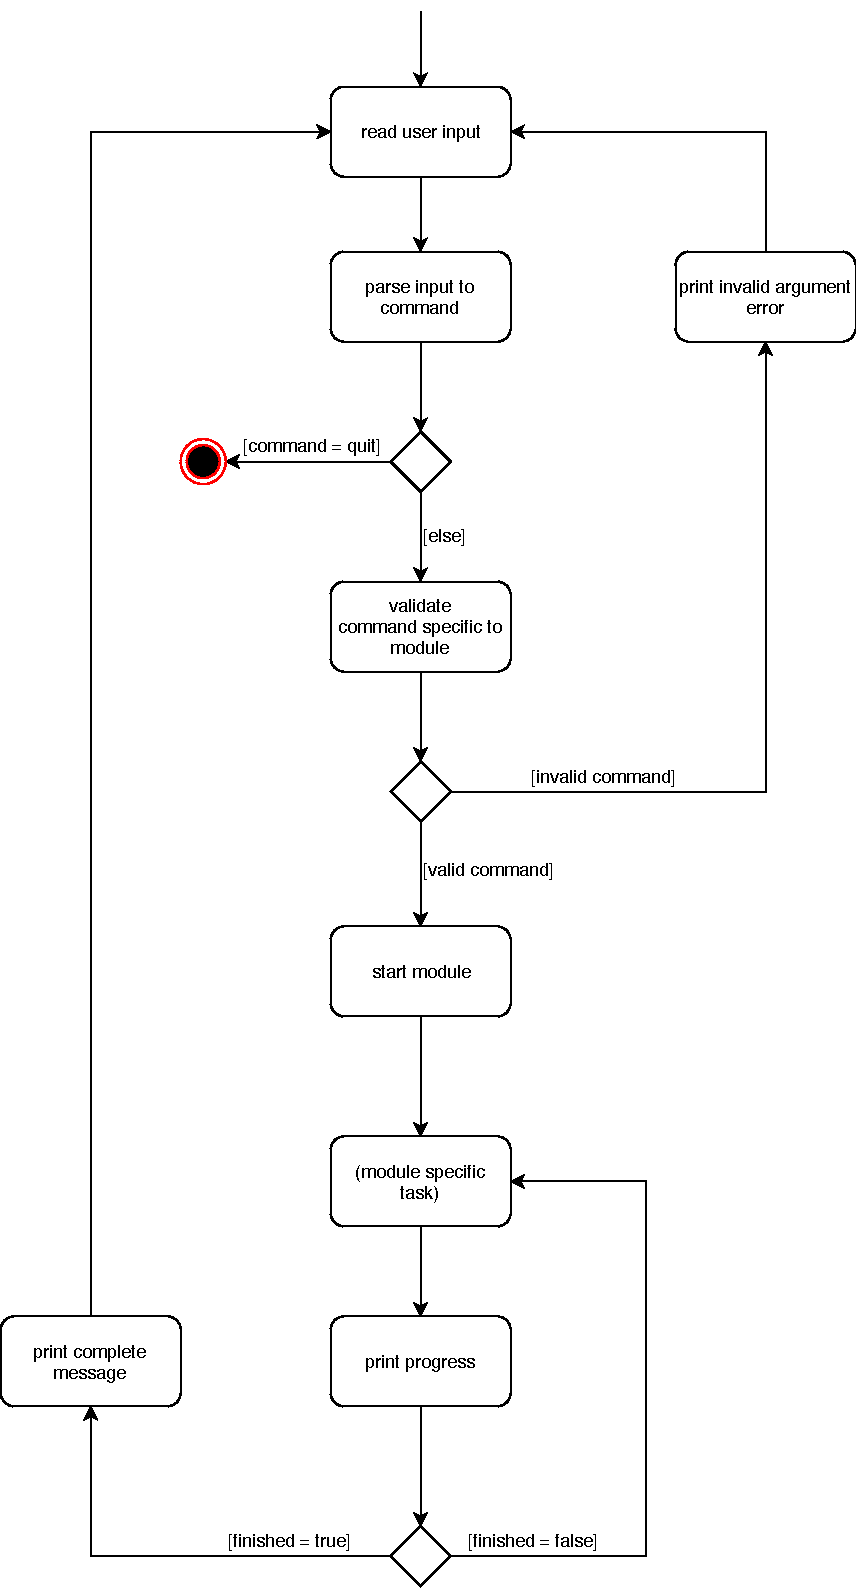
\includepdf[pages={1}]{ActivityDiagrams/PDF/user_input_activity_diagram}

This activity diagram shows the main workflow of the whole program.
The program first waits for user input.
After the user enters his input into the command line interface, the CommandParser parses this input to a command.
If the command equals quit, the programm will exit.
If not the command will be validated to contain enough information to start the desired module.
If it is not valid, an error message will be printed and the user can enter a new input.
If the command is valid, the module will be started.
Therefore the module computes his specific task in iterations.
After each iteration it print the current progress to the user.
This two activities repeat until all tasks are done.
When the module is finished, the program prints a complete message and start waiting for new user input.

\subsection{Class Diagrams}

\subsubsection{Command Parsing}

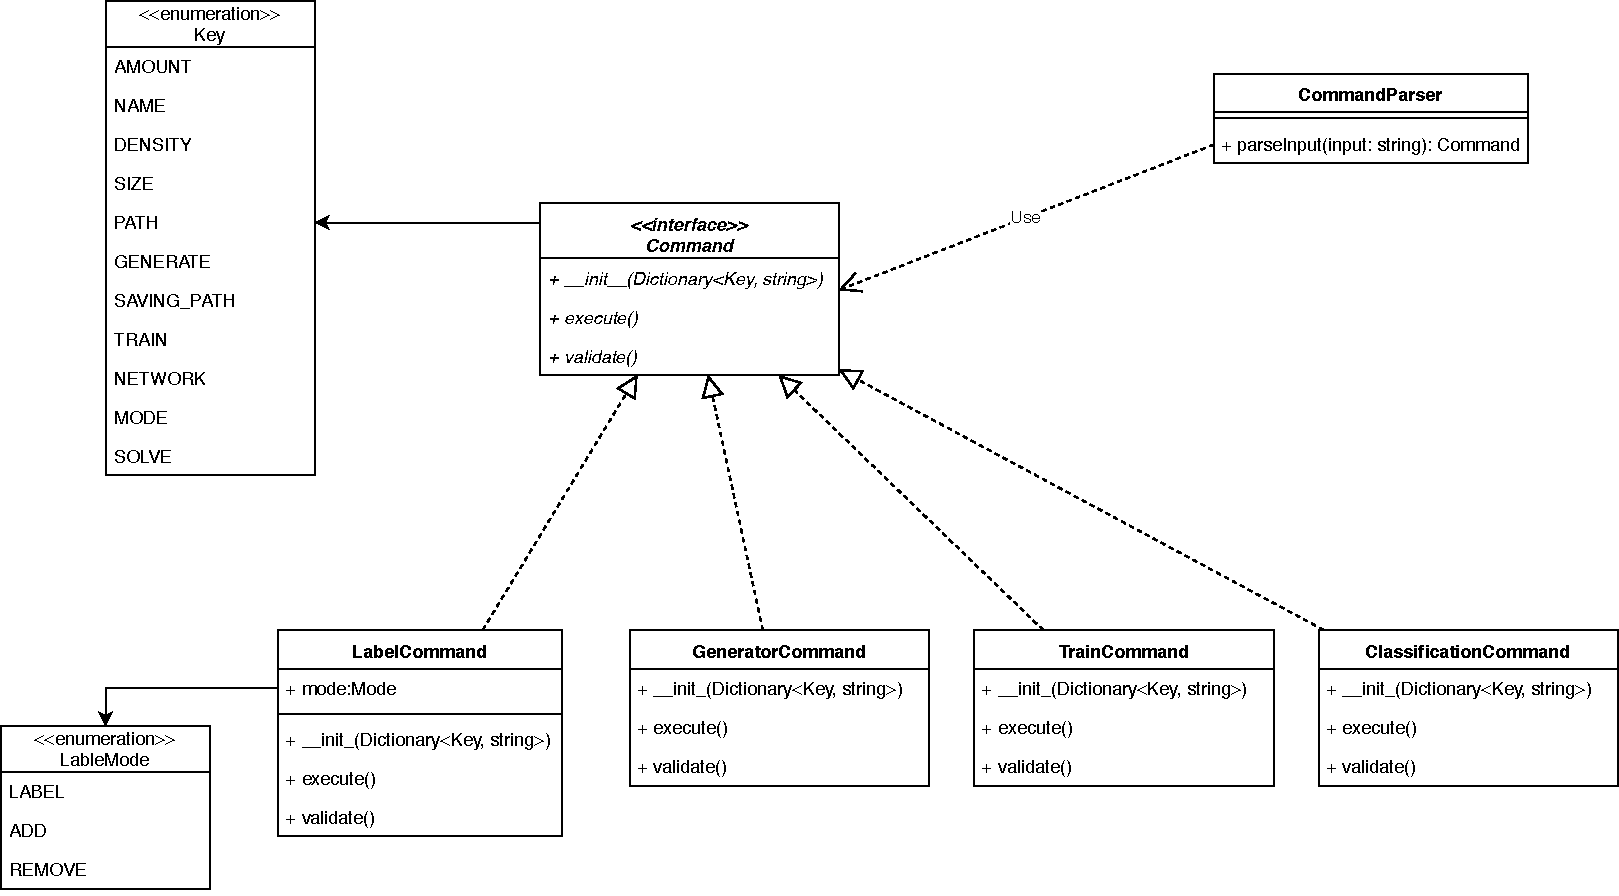
\includepdf[pages={1}]{ClassDiagrams/PDF/CommandParsing}

This class diagrams shows all classes that are used by the CommandParser.
The CommandParser has one method that receives an input string and returns a command.
This method uses the first word of the input string to determine which module is supposed to be started.
Based on this he creates an instance of this subclass of the command.
The remaining string will be parsed to a dictionary with keys and values. 
This dictionary is passed to the constructor of the command object.
In the constructor of the command, the command also calls the validate() method.
This method checks if all arguments that are necessary for the specific module start are provided.
After that is finished the command can be returned by the CommandParser.
The execute method of the command can be then used to start the modules computation.

\subsection{Component Diagrams}

\subsubsection{Component Interaction Overview}

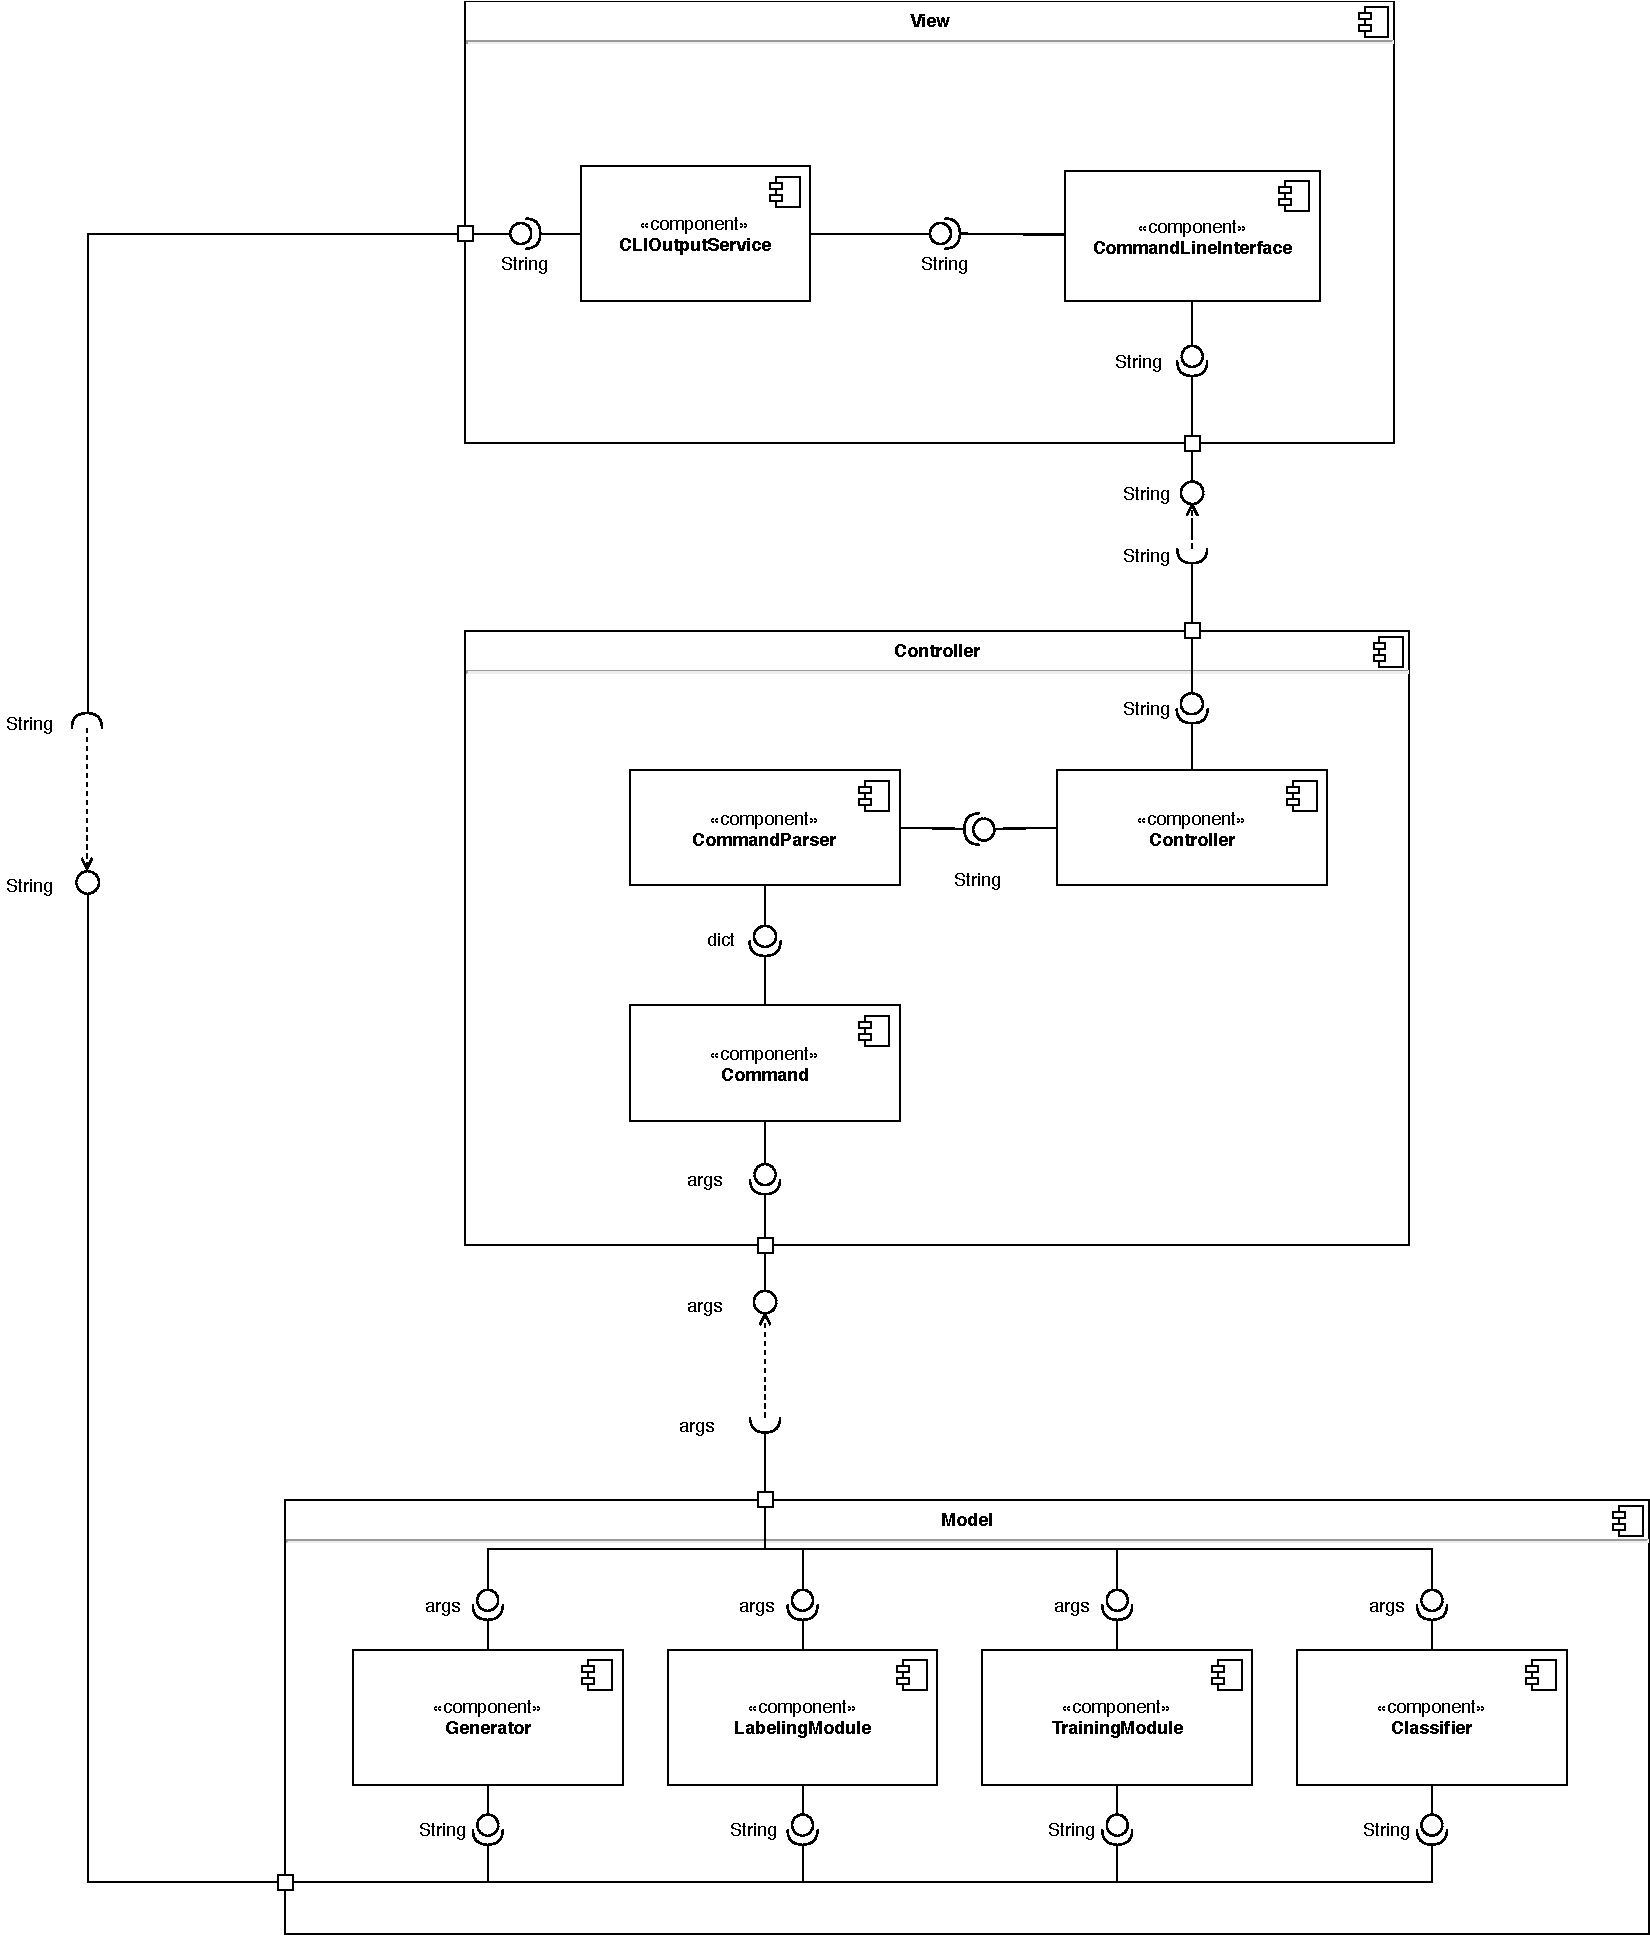
\includepdf[pages={1}]{ComponentDiagrams/PDF/interaction_overview}



\subsection{Sequence Diagrams}


\section{Collector}

\subsection{Class Description}

\subsubsection{Class Collector}
The Collector class is responsible for collecting a given amount of matrices and saving it into a HDF5 dataset.
When the user types collect into the CLI, a collector Object will be created and the public method collect() with its parameters:
amount, name, size, density and path will be called. The class has a Saver class attribute and a Generator class attribute.
It uses methods from the Generator class to get matrices to collect and methods from the Saver class to save the collected dataset.
(see the collect method Activity Diagram for a more detailed overview).
The Collector class is the interface between matrix collecting and the CLI and conceals all the classes of the Collector described in the following.

\subsubsection{Class Saver}
The Saver class is just responsible for saving a given matrix dataset.
Its only method is the save(dataset, name, path) method, which
is called by the collect method from an Collector object.
The save method takes an NPArray as a matrix dataset, converts it into an HDF5 file and saves it into a given directory with a given name.

\subsubsection{Class Generator}
The Generator class is responsible for actually generating matrices by transforming raw matrices from SuiteSparse and validating them.
The generate(size, density):Matrix method is called by a Collector object, uses the Matrix class to initialize an empty matrix, uses the Ssget class to fetch and transform matrices from the SuiteSparse collection and uses the static Validator.validate method to check if the matrix is regular and can be returned.

\subsubsection{Class Ssget}
The Ssget class is responsible for fetching matrices from the SuiteSparse collection, transforming them and returning them.
Its getMatrix method is called by a generator object.
The getMatrix method uses the Matrix class to initialize a matrix, then the private downloadMatrix method to fetch a matrix from SuiteSparse, and after that uses its private cutMatrix method to cut a fixed size, regular matrix out of it.

\subsubsection{Class Validator}
The Validator class is a util class and responsible for validating given matrices(checking for regularity)
 Its only static method validate takes a matrix and returns true for regular, and false for not regular.

\subsection{Activity Diagrams}

\subsection{Class Diagrams}

\subsection{Sequence Diagrams}


\section{Labeling Module}

\subsection{Class Description}

\section{Training Moulde}

\subsection{Class Description}

\subsubsection{Class Configuration File}
The configuration file is a text file.
It is used to specify all necessary information the class neural network needs to train the neural network.
If the user does not change anything in the configuration file, defaut options will be used.The configuration file is organized in four main categories. 
\begin{enumerate}
\item loading path of the set of matrices 
\item saving path for the neural network
\item loading path for the neural network
\item model definition and hyperparameters abc
\end{enumerate}
The loading path of the set of matrices is the path in which the matrices that are used for the training and testing are stored.
The training module only supports one hd5 file.
If the path is any other file, the labling module will print an error(would crashing make sense if the user has to change the config file anyway?).
For the training and testing making sense there should be at least 500 matrices in the hd5 file.
Otherwise the accuracy of the neural network will be so low that i can not be used for classification.
If there is no path specified, the training module will use a default path.
In the default path will be the latest matrices that the labling module has produced. \newline

The saving path for the neural network is the path where the trained and tested neural network will be safed.
It will be safed as a Keras model.
If there is no path specified, the neural network will be safed at a default destination.
If there is no path for the neural network specified in the module Classifier the module will use this default path to load its neural network.\newline

The loading path for the neural network is strictly optional.
If this path is specified the training module will use the neural network in the path for training and testing.
This option enables the user to use a pre-trained neural network for training.
This could be the case if the user interrupts the training process at a certain time and wants to to repeat the training later.
Other use cases are of course possible too.
The neural network has to be a model of the Keras framework. If the path is any other file the training module will print an error(crash?).
If this path is not specified the training module will create a new neural network(with the model definition and hyperparamters of the next category) and train with it. \newline

The model definition and hyperparameters are used to determine which neural network will be trained and tested. The model definition determines the following:
\begin{itemize}
\item the amount of layers
\item the amount of nodes in every layer
\item the kind of neural network(e.g. Convolutional)
\item the activation function
\item the regularization
\end{itemize}

The hyperparamters determine the following:

\begin{itemize}
\item the dropout
\item the batch size
\item how much of the data should be training and how much should be testing data
\end{itemize}

\subsubsection{Class TrainingModule}
The TrainingModule class is responsible for the training and testing of a neural network.
It can not be instantiated, since it is a utility class.The structure is mainly oriented towards the keras workflow and will be further described later.
The class offers one public method, the method train(). \newline
When the user types train() in the CLI the method train in the class TrainingModule will be executed in the following manner(see the activity diagram for a graphical overview).
\begin{itemize}
\item load the configuration file
\item load the matrices
\item seperate matrices in training and test data
\item train a preexisting neural network or a new one(depending on the configuration file)
\item test the neural network
\item save the neural network
\end{itemize}

The configuration file that gets loaded will be used to specify the subsequent points.\newline

The configuration file will determine from which path the labeled matrices will be loaded.
If there were no changes made in the configuration file, the default path will be used(see the class description of the configuration file).
The labeled matrices will be loaded in one hd5 file. If the path links to any other file, the class TrainingModule will print an error to the command line (crash?). \newline

After that the class TrainingModule will seperate the training and test data.
How the data will be seperated is specified in the configuration file.\newline

Following there are two alternatives
 If the user has specified a neural network in the configuration file, the class TrainingModule will train this neural network with the labeled matrices for the training.
If the user has not specified a neural network in the configuration file, the class TrainingModule will create a new neural network with the specifications in the configuration file.
If there are no model definitions in the configuration file the class TrainingModule will use the default neural network(see default neural network).
The class TrainingModule then proceeds with training the new neural network with the labeled matrices for the training. In both cases the current loss will be continously printed to the command line.\newline

Now the neural network is trained. The class TrainingModule proceeds with testing the neural network with the labeled matrices for the testing.
This process will determine the accuracy of the neural network on the given test matrices.
The accuracy will be printed on the command line.\newline

After that the neural network will be safed as a keras model.
The path for the saving is specified in the configuration file.

\subsection{Activity Diagrams}

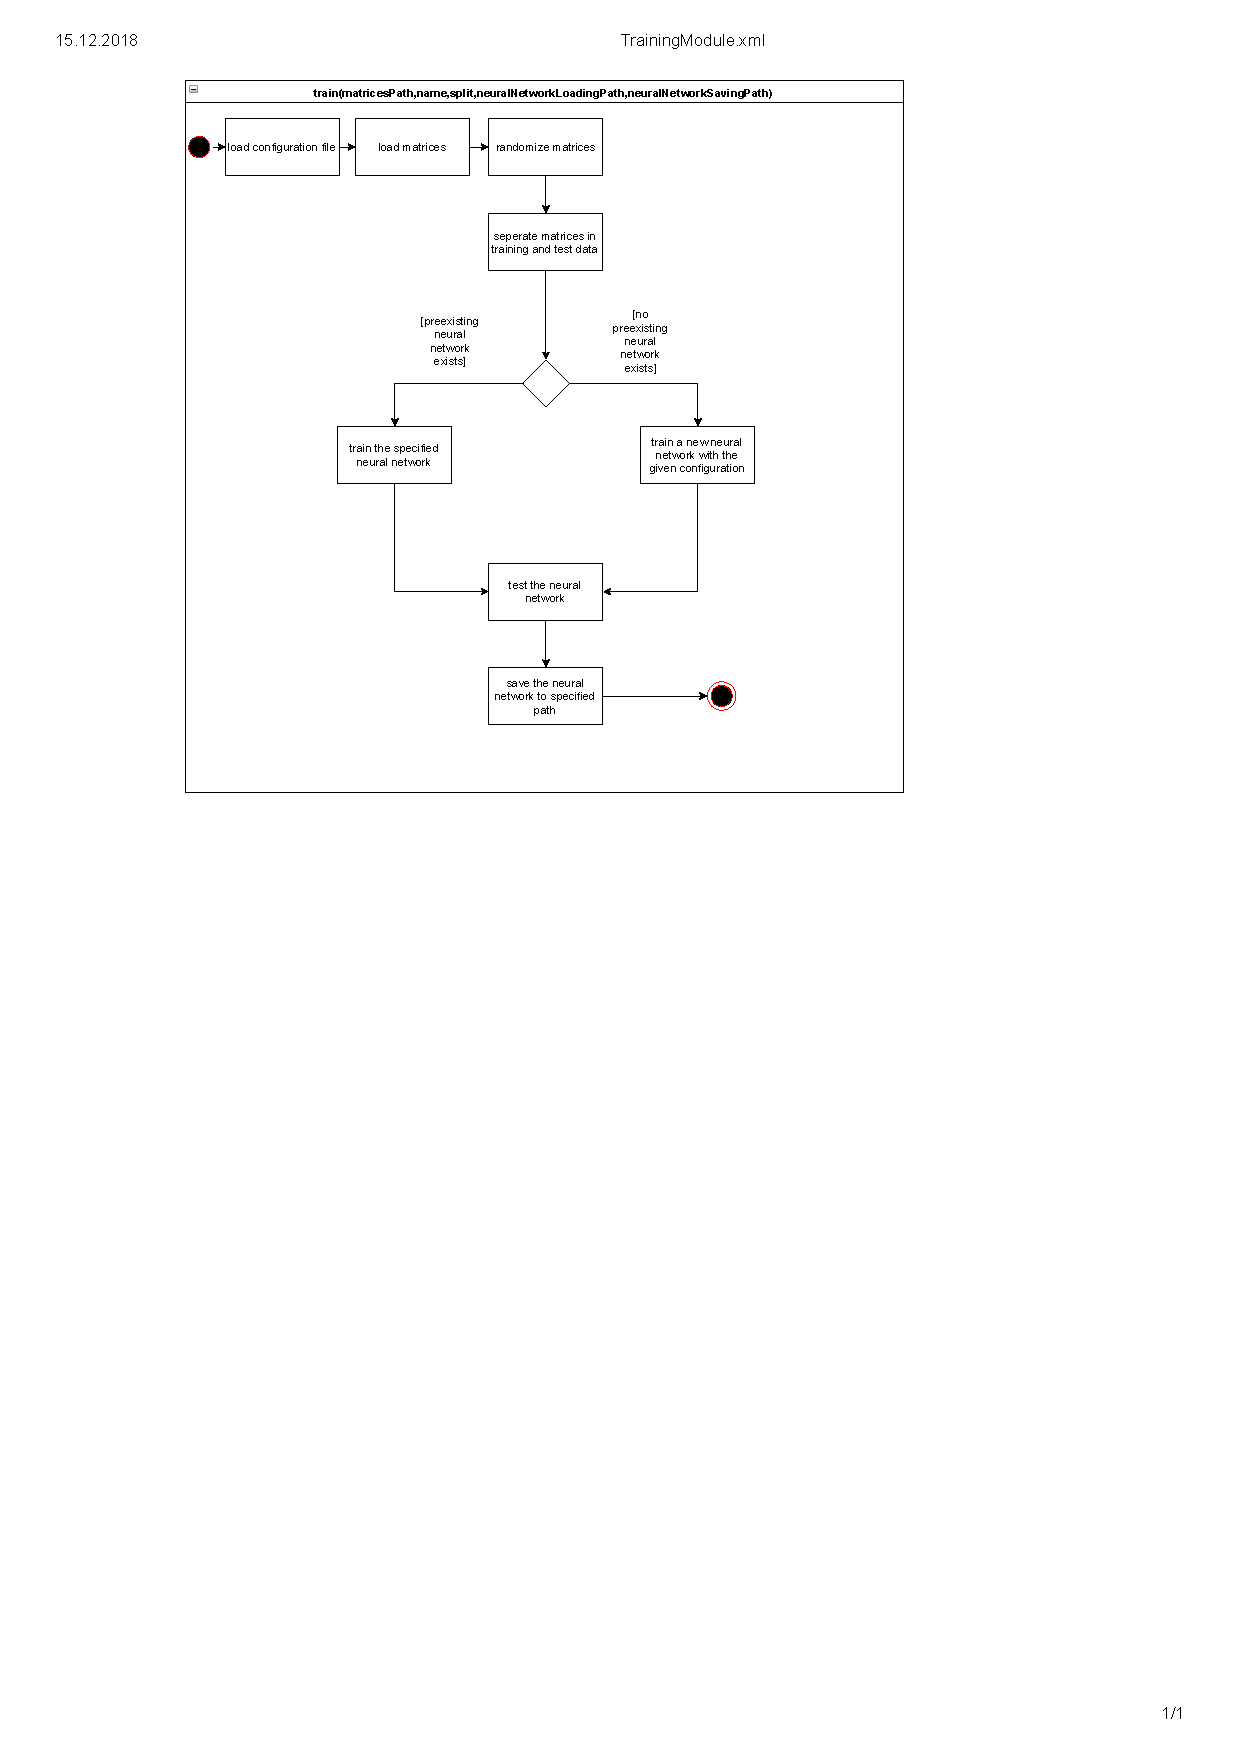
\includepdf[pages={1}]{ActivityDiagrams/PDF/TrainingModule}

\subsection{Class Diagrams}

\subsection{Sequence Diagrams}


\section{Classifier}
The classifier classifies a matrix given by a path. 
In this path, the matrix is stored in the form of an HDF5 file.
As a second parameter the neural network path will be given. 
In this path the trained network the user wants to use for his classification is saved.
As a last parameter the user can set the solve flag, what gives the opportunity to also solve the matrix with the best solving algorithm classified by the neural network.




\subsection{Class Descriptions}

\subsubsection{Class Classifier}
\subsubsection{Interface Algorithm}
This interface is for the different algorithms for solving a given matrix.
\subsubsection{Class ConcreteAlgorithm}
The Concrete Algorithm class is for solving a matrix in a certain way.
This means a certain approach to solve a matrix.
\subsubsection{Class Matrix}

\subsection{Class Loader}

\subsubsection{Class Validator}
The Validator class is a util class and responsible for validating given matrices(checking for regularity)
Its only static method validate takes a matrix and returns true for regular, and false for not regular.

\subsubsection{Class Neural Network}

\subsection{Activity Diagrams}

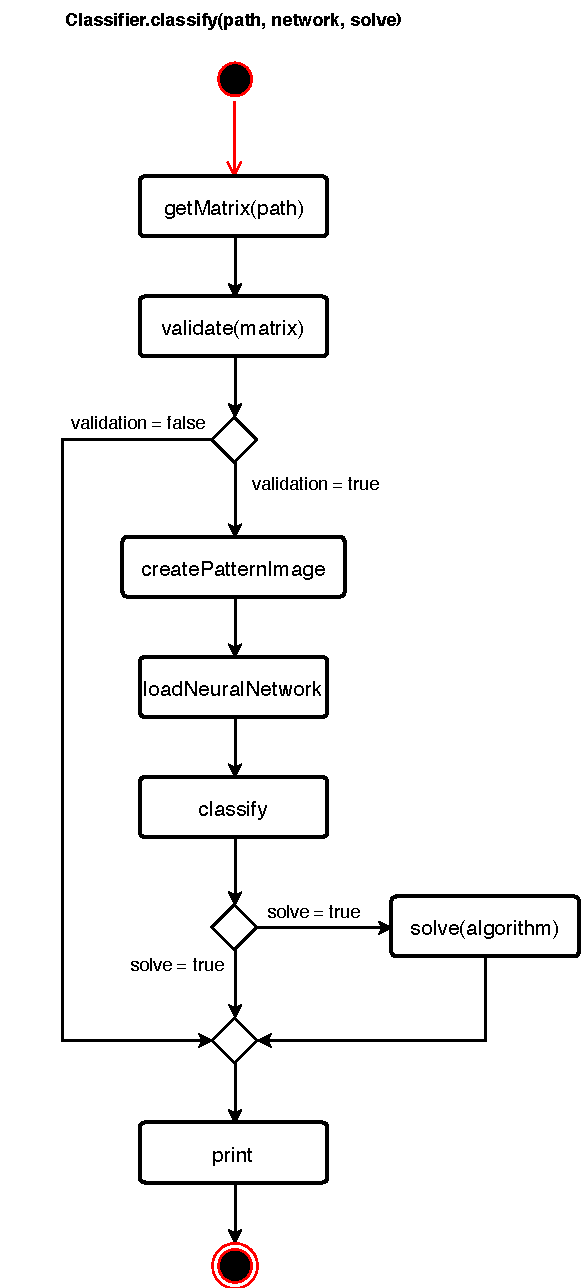
\includepdf[pages={1}]{ActivityDiagrams/PDF/classification}

\subsection{Class Diagrams}

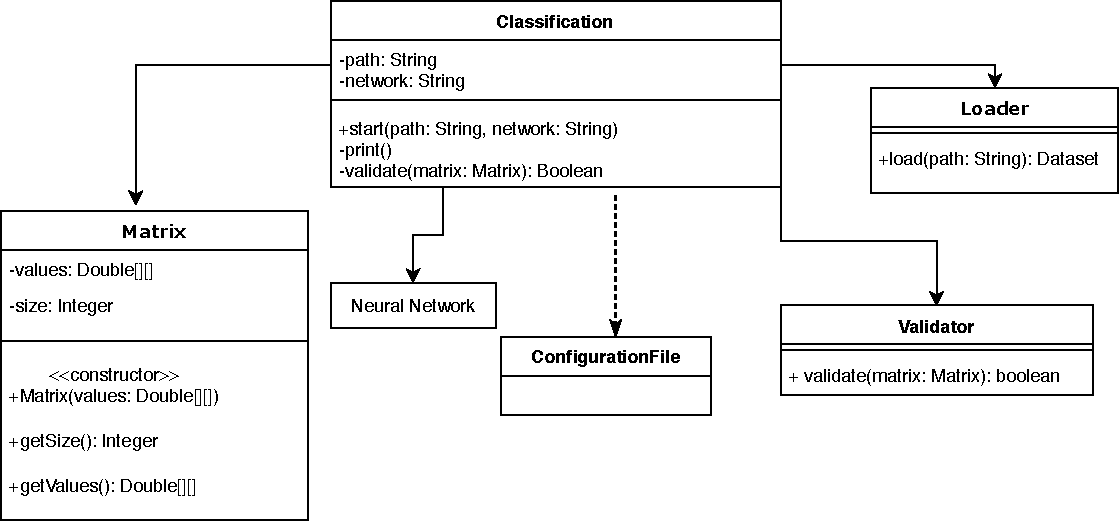
\includepdf[pages={1}]{ClassDiagrams/PDF/Classifier}

\subsection{Sequence Diagrams}

\section{Explanations}
\subsection{default neural network}
how is the nn structured(layers,activation function), what is it trying to achieve,...

\section{Glossary}
%\glspl{collector}, labeling modle, neural network, classifier, default settings  \glspl{Dateiformat}

% % Automatisch generiertes Glossar (Latex zwei mal ausführen um Glossar anzuzeigen)
%
%\glsaddall % das sorgt dafür, dass alles Glossareinträge gedruckt werden, nicht nur die verwendeten. Das sollte nicht nötig sein!
\printnoidxglossaries

\end{document}
